\section{Calculating complexity in relational algebra}
\label{sect:method:complexity}
A method for indicating complexity of relational algebra trees was suggested
by \O ystein Torbj\o rnsen at Fast Search \& Transfer. This method is based on the assumption
that the algebra will be executed on an implementation written in Java or a
similar object oriented language. Not withstanding the
benefits of compile-level optimisations and other ways to increase performance
such as caching, this method of complexity indication defines complexity as
creation of new objects in run-time, and the cost of sort and join operations.

This definition of complexity does \textit{not} account
for disk I/O, nor is it a direct measurement of performance. However, given
an algebra tree which is to be executed on some known host implementation, it
may give an indication of spending of time and computational resources.

\subsection{Tuple and field creation}

\begin{myDefinition}
A \textbf{field} is an in-memory object which contains a value and a mapping to
an attribute name in a relation
\label{definition:relalg_field}
\end{myDefinition}

\begin{myDefinition}
A \textbf{tuple} is defined as an in-memory object which contains a set of
\textit{fields} (definition \ref{definition:relalg_field}), where each field
contains a value for some given attribute in the relation
\label{definition:relalg_tuple}
\end{myDefinition}

\begin{figure}[!htp]
\begin{center}
  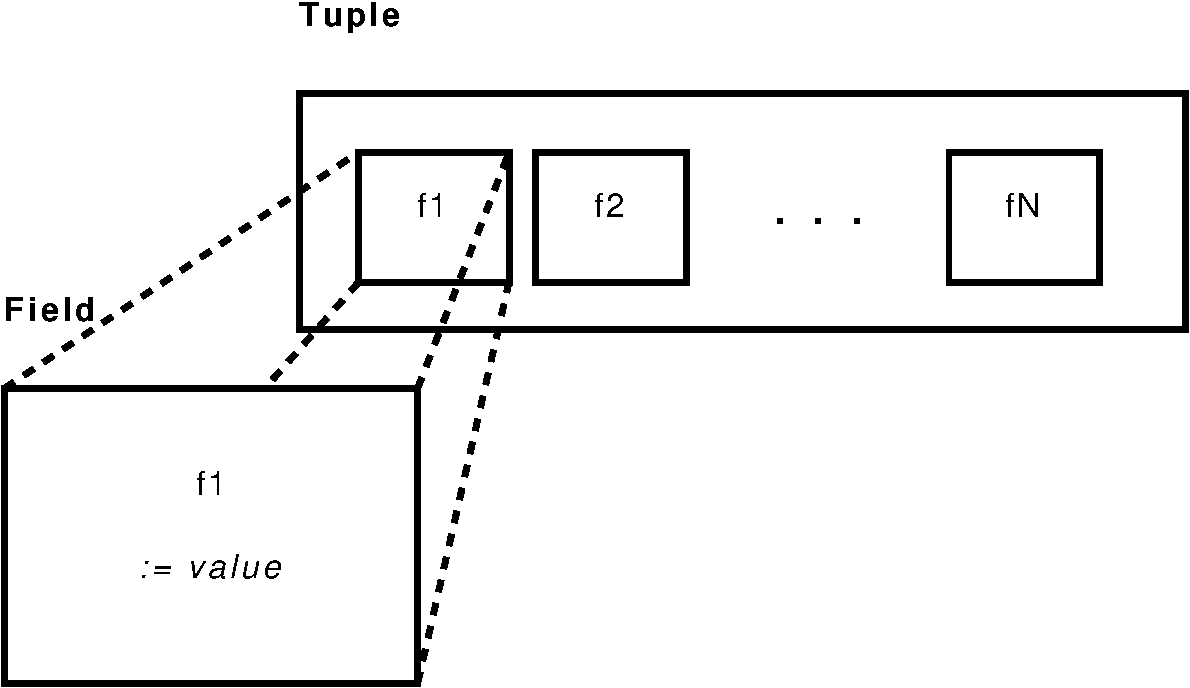
\includegraphics[width=0.65\textwidth]{diagrams/tuple_post}
  \caption[Tuple/Field structure]{The structure of a \textit{tuple} with
  \textit{fields}}
  \label{fig:method:tuple_field}
\end{center}
\end{figure}

\subsubsection{Semantics}
A new tuple is assumed to be created every time an old tuple needs to add or
remove one or more fields. A new field is assumed to be created for every new
value for any attribute for any tuple.

\subsubsection{Implications of semantics}
Any kind of projection of $x$ tuples over $n$ ``new'' attributes and $o$
``old'' attributes generates $x$ new tuples and $n$ new fields (note that
duplicates are not removed). Old fields are reused, and attribute renaming
is naturally capable of reusing old fields.

Any kind of tuple construction (e.g using the \textsf{make()} operator)
for $n$ tuples and $m$ fields generates $n$ new tuples and $n \times m$ new
fields.

\subsubsection{Assumptions}
\label{sect:method:complexity:assumptions}
Pathfinder generates relational algebra which contains some operators for which
the behaviour is unknown. Some assumptions have made about these operators:
\begin{itemize}
  \item The \texttt{Join} operator is assumed to produce $n*m$ fields for an
  input of $n$ tuples and $m$ fields
  \item The behaviour of the \texttt{Diff} operator is unknown, it is assumed
  to produce 0 tuples and 0 fields
  \item The behaviour of the \texttt{Distinct} operator is unknown, in favour
  of Pathfinder it is then assumed to produce 0 tuples and 0 fields
  \item The \texttt{Not} operator is assumed to perform an inversion of boolean
  values and thus produces $n$ tuples and $m$ fields for an input of $n$ tuples
  and $m$ fields (where $m$ is always 1 in the comparisons made in this dissertation)
  \item The \texttt{Cast} operator is assumed to produce $n$ tuples and 1
  field for an input of $n$ tuples and $m$ fields
  \item The \texttt{Attach} operator is assumed to produce $n$ tuples and $m$
  fields, where $m$ is the number of fields constructed by the \texttt{Attach}
  operator and $n$ is the number of input tuples
\end{itemize}

\subsection{Join and sort tuple I/O}
\begin{myDefinition}
The \textbf{input} of an operator is defined as the sum of tuples \emph{entering} the
operator
\label{definition:relalg_input}
\end{myDefinition}

\begin{myDefinition}
The \textbf{output} of an operator is defined as the sum of the tuples \emph{produced}
by the operator
\label{definition:relalg_output}
\end{myDefinition}

\subsubsection{Semantics}
For every operator that either performs a join or sort operation, the number of
\textit{input} and \textit{output} tuples are counted. The minimum, maximum,
and averages are calculated for both \textit{input} and \textit{output}.

\subsection{Total complexity}
\begin{myDefinition}
Measurement of \textbf{complexity} is defined as that for some given
operator $\alpha$, counting the following:
\begin{itemize}
  \item Creation of new \textbf{tuples} (definition
  \ref{definition:relalg_tuple})
  \item Creation of new \textbf{fields} (definition
  \ref{definition:relalg_field})
  \item If $\alpha$ performs a sort or join operation, all
  \textbf{input}(definition \ref{definition:relalg_input}) and \textbf{output}
  (definition \ref{definition:relalg_output}) tuples
\end{itemize}
The integer sum of counting field and tuple creations (from and including 1 and
up) defines the \textbf{complexity} for $\alpha$. Further, the
sum of all the complexity sums in some given relational algebra tree defines the
\textbf{complexity sum} for that given tree. Additionally, the minimum, maximum
and average \textit{input} and \textit{output} tuples defines the
\textbf{tuple I/O complexity} for that given tree.
\label{definition:relalg_complexity}
\end{myDefinition}
